%========================================================================================%
%					NOTE
%========================================================================================%
% Probably this theme will not compile with standard pdftolatex compiler due to lack of some 
% fonts used in the theme. It is recommended to compile with XeLaTex instead.

% !TEX program = xelatex

%========================================================================================%
%					DOCUMENT SETUP
%========================================================================================%
\documentclass{beamer} 
\usetheme[progressbar=frametitle]{metropolis}

\usepackage{textpos}

\usepackage{amsmath}

\usepackage{mathrsfs}


%For making diagram and drawing
% \usepackage{tikz}
% \usetikzlibrary{shapes,arrows, fit, positioning}

%For appendix
\usepackage{appendixnumberbeamer}


\usepackage[export]{adjustbox}

%Some additional graphcs tools
\usepackage{graphicx}
%\usepackage{datatool}
%\usepackage{animate}

% For someone using the pgfplot tools
%\usepackage{pgfplots}
%\usepgfplotslibrary{dateplot, groupplots}
%\pgfplotsset{compat=1.14}
%\usepgfplotslibrary{fillbetween}

%Remove words break, wrap instead
\usepackage[none]{hyphenat}


%for custom date
\usepackage[english]{babel}
\usepackage[nodayofweek,level]{datetime}

\usepackage{xspace}
\newcommand{\themename}{\textbf{\textsc{metropolis}}\xspace}

\renewcommand*{\arraystretch}{1.2}

\usefonttheme[onlymath]{serif}




%===================================================================================%
%				FRONT PAGE
%===================================================================================%
\titlegraphic{%
\hfill%

\includegraphics[height=1.5cm, valign=c]{logos/ccfd3.png}%
\hspace{15pt}%

\includegraphics[height=1.5cm, valign=c]{logos/symbol-PL.pdf}%
}

\title{Introduction to concurrency in modern C++}

\date{\vspace{5pt}\formatdate{13}{1}{2021}}

%===================================================================================%
%				THEME COLORS
%===================================================================================%
% specify main colors which are being used by the theme
\definecolor{bordercolor}{HTML}{002699}
\definecolor{fillcolor}{HTML}{002699}

% fix theme black color which affects tikz plots
\definecolor{black}{RGB}{0,0,0}




%===================================================================================%
%				ACTUAL DOCUMENT CONTENT
%===================================================================================%

\begin{document}

\maketitle

%force to add logos to the each frame title
\addtobeamertemplate{frametitle}{}{%
\begin{textblock*}{100mm}(.9\textwidth,-0.9cm)

\includegraphics[height=0.8cm, valign=c]{logos/ccfd3_white.png}\hspace{10pt}
\includegraphics[height=0.78cm, valign=c]{logos/symbol-PL-white.pdf}
\end{textblock*}}

\begin{frame}{Disclaimer}
\begin{enumerate}
\item This will be a fire hose talk
\item Despite this, we are only going to scratch the surface
\end{enumerate}

\includegraphics[width=\linewidth]{firehose.png}
\end{frame}

\begin{frame}{Multithreading}
\begin{itemize}
\item Concurrency: when tasks start, run, and complete in overlapping time periods
\item Parallelism: when two or more tasks execute simultaneously
\item How do we get there? Start a new thread for each task?
\item Lets try to design a task system...
\end{itemize}
\end{frame}

\begin{frame}{Multithreading}
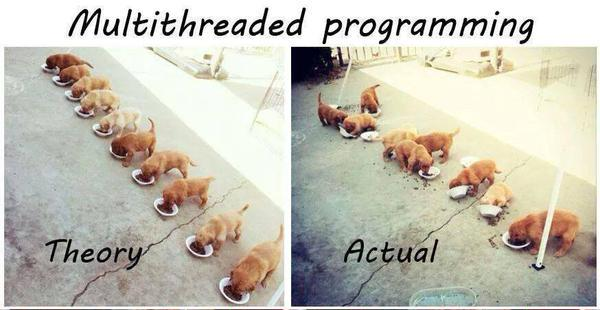
\includegraphics[width=\linewidth]{concurrency.jpeg}
\end{frame}

\begin{frame}{Task Queue}
\begin{itemize}
\item Task = Callable + Arguments
\item Task queue stores tasks and executes them in FIFO order on a thread pool
\item API:
\begin{itemize}
\item[>] push(f, args...)
\item[>] complete()
\end{itemize}
\item Performance!
\item Let's take a look at Sean Parent's talk for some inspiration...
\end{itemize}
\end{frame}

\begin{frame}[standout]
The features...
\end{frame}

\begin{frame}{Variadic templates}
\begin{itemize}
\item Lets us write templates with an unspecified number of parameters
\item Syntax: \texttt{template < typename ...T >}
\item The above can be instantiated with any number of types (including zero)
\item \texttt{T} is a parameter pack and must be expanded whenever used
\end{itemize}
\end{frame}

\appendix
\begin{frame}{Q\&A}
    \alert{Thanks for listening}
\end{frame}
\end{document}
